% vim:set ft=tex:
\section{Fiasco.OC \& L4Re}
\label{state:env}
The related research I present in section \ref{state:related} states the
following feature requirements:
hardware performance counters, assignment of threads to specific
cores, and the ability to overrule the kernel scheduler.

Fiasco.OC is a µ-kernel of the L4-family and follows the design paradigm to
only implement mechanisms in the kernel and no policies.
For performance reasons, the scheduling policy is the only policy implemented in
the kernel.
The scheduling parameters in a scheduling request from user land consist of
a priority level, a time slice size request and a descriptor stating on which
cores the thread wants to be scheduled.
The kernel schedules the thread on the first available core in the descriptor,
checks if the priority level is in a valid range, and assigns a time
quantum.
It does neither balance the amount of threads per core, nor prevent
oversubscription.
However, it provides the mechanism to design a more sophisticated load
distribution scheme as a user-level service.

OC in Fiasco.OC stands for object capability, a system providing a thread local
namespace for references to other objects, such as the scheduler, object
factory, and memory management.
A new task populates its capability space with a set of capabilities inherited
from its parent to be able to interact with the system.
This set is completely independent of its parent capability namespace; parent
and child can replace capabilities in their capability space without affecting
the other.
This property enables the use of proxies, implementing the same interface, but
a different policy on top of the base service.
An object registers the new service in its capability space.
So different services can be implemented on top of each other, providing
different policies for subhierarchies of the object space.


The L4 runtime environment provides a scheduling service skeleton, which
defines the kernel and user interface.
Using this skeleton and the capability namespace property, a scheduling service
can replace the default L4Re scheduler and implement further analysis of each
thread.
The skeleton also enables thread-specific proxies with an individual
configuration.
This mechanism will be used in this work.
\\

Regarding hardware performance counters, the kernel provides neither a system
call interface to read or configure them, nor per thread accounting of
configured counters.
Access to hardware performance counters is critical for this project, so I need
to implement a mechanism to provide this for a user-level service.



\begin{comment}
\textbf{Fiasco.OC}
\begin{itemize}
  \item Kernel scheduler does no balancing, assigns thread to the first
    core specified in the affinity descriptor
  \item affinity descriptor: core(s) a thread should run on
  \item Syscall via run\_thread() to pass affinity descr to kernel scheduler
  \item interface to query execution time for each thread
  \item capability system -- to derive communication relationships from
  \item	Kernel feature wishes derived from related work: Performance counters
    and per thread accounting
\end{itemize}

\textbf{L4Re}
\begin{itemize}
  \item provides scheduler proxy interface, including affinity descriptor,
    scheduling parameters
  \item syscall interface
\end{itemize}
\end{comment}


% -----------------------------------------------------------------------------

\section{\gls{intel} Haswell Architecture}
\label{state:haswell}

In section \ref{state:related}, I mentione several hardware features.
The most important of all are performance counters to measure cache misses,
cycles and instructions executed.
The performance counters in the target processor --- an \gls{intel} Haswell
generation Core i7-4660K -- are able to count these three events and many more.
The processor contains Architectural Performance Monitoring version 3
capabilities, which consist, among other features, of three fixed-function
performance counters counting Instruction Retired, Unhalted Core Cycles, and
Reference Instruction Retired (\cite{intel_arch_ref_manual_2015}).
In contrast to the first two counters, the last counter is unaffected by
processor speed changes due to power saving or \textit{turbo boost} features.

Besides these, four general purpose performance counters are available per
logical core, which can be programmed to count one specific event.
All \gls{intel} Core i generations support architectural performance monitoring
in different versions, but all versions are guaranteed to support the following
events:
Unhalted Core Cycles, Instruction Retired, Unhalted Reference Cycles,
LLC Reference, LLC Misses, Branch Instruction Retired,
and Branch Misses Retired (\cite{intel_arch_ref_manual_2015}).

Besides these central events, each hardware generation supports a different set
of so-called ``non-architectural performance events''.
This non-architectural event set allows to monitor many specific events, e.g.
L2-misses/-hits, micro-ops per logical core executed per cycle, or unhalted
core cycles executed in ring 0.

Another difference to the target processor, compared to most processors used in
earlier research, is the \gls{smp} architecture.
In contrast to \gls{cmp}, the architecture does not define cache groups,
because the \gls{llc} is shared among all cores.
Figure \ref{state:fig:core_layout} shows an example of the cache hierarchy of
the \gls{intel} Haswell processor.
Each core consists of two \gls{ht} cores, sharing L1- and L2-caches.
All cores on one socket share the same \gls{llc}.
The \gls{llc} is inclusive, meaning each cache line present in L1I-, L1D-, or
L2-cache is also present in the \gls{llc}
(\cite[2-23]{intel_optimization_manual_2015}).
This eases the lookup of cache lines in other cores on the same package.
If the line is present in the \gls{llc} the cache-coherency status indicates,
if and in which core's caches it is present.

%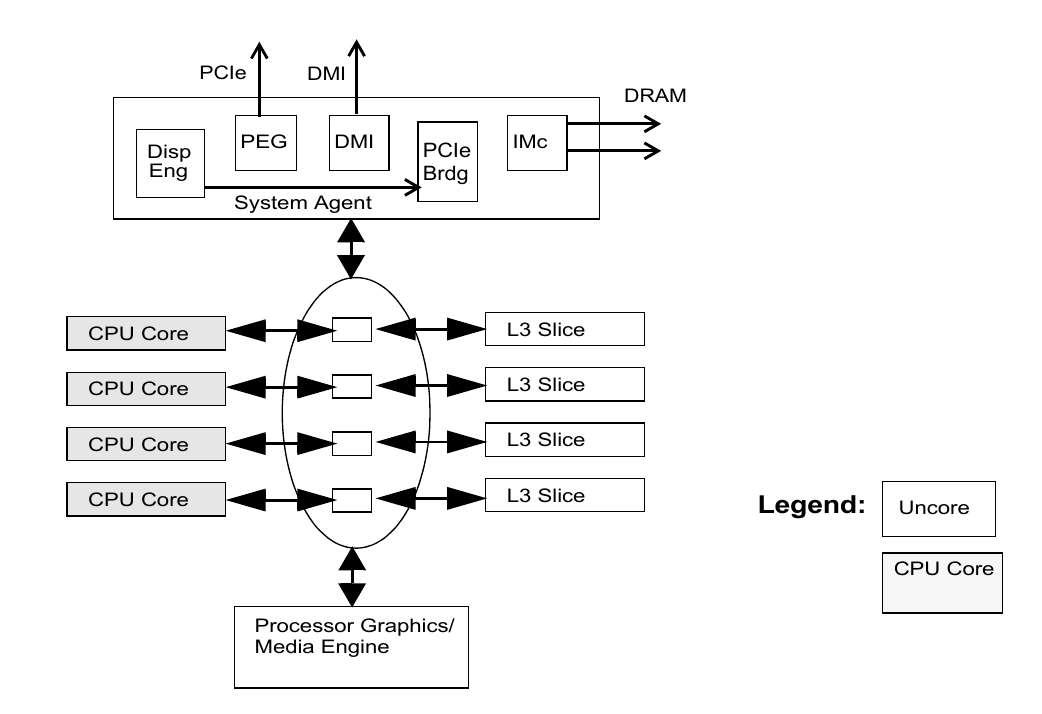
\includegraphics[width=0.8\textwidth]{images/haswell_architecture_by_intel_large}

\begin{figure}[h!]
  \setcapindent*{1em}
  \begin{captionbeside}[]{Schematic layout of two cores of a Core i7-4660K quad-core.
    Each physical core has two logical cores sharing the core's L1I-,
    L1D-, and L2-cache.}
  \includestandalone[mode=tex,width=0.65\textwidth]{images/haswell_core_layout}
\end{captionbeside}
  \label{state:fig:core_layout}
\end{figure}

\paragraph{Topology analysis.}
The topology of the CPU can be determined at run-time.
It is useful to detect which two logical cores exist together on the same
physical core, since Fiasco boots the physical cores in a nondeterministic order.
The CPU provides this information through the CPUID interface, if the
extended topology enumeration leaf is supported(\cite[Vol.2A
3-179]{intel_arch_ref_manual_2015}). This is the case for the
target CPU.

\begin{comment}
\begin{itemize}
  \item diagram of architecture: four cores with L1I/D \& L2 cache; two smt/ht
    cores per physical core; L3 cache shared and sliced, ring buffer for
    access; mem controler in uncore package;
  \item 4 prefetcher per cache; 2 for L1D, 2 for L2 cache
  \item L1D \& L2 cache data is present in L3 cache to be able to redirect
    requests from other cores to the correct cache. --> Issue with security; no
    cache side attack surface reduction
  \item IF security: dual socket system with one core dedicated to security
    tasks for an interval
  \item L3 cache slices corespond to number of cores
  \item logic portion and data array portion; access, coherency, memory
    ordering, LLC misses, writeback to memory; cache lines
  \item hash function uniformly distributes addresses
  \item access times to L3 cache varies depending on travel distance on the
    bi-directional ring buffer
  \item system agent receives memory requests not serviced by cache and
    redirects to IMC
\end{itemize}
\end{comment}

% -----------------------------------------------------------------------------
